\section{Schwellenwert und Kosten}
\label{sec:schwelle}

Bei einem Ausfallanteil von 26,1~\% ist die Schwelle
0,5 willkuerlich. Sie wird hier aus dem erwarteten Nutzen abgeleitet:

\begin{table}[H]
  \centering
  \small
  \begin{tabular}{lrrrrrr}
    \toprule
    Schwelle & Precision & Recall & F1 & TP & FP & FN \\
    \midrule
    0,5 (Standard) & 0,526 & 0,781 & 0,629 & 143 & 129 & 40 \\
    1:1 & 0,650 & 0,628 & 0,639 & 115 & 62 & 68 \\
    5:1 & 0,495 & 0,880 & 0,634 & 161 & 164 & 22 \\
    10:1 & 0,394 & 0,945 & 0,556 & 173 & 266 & 10 \\
    50:1 & 0,322 & 0,995 & 0,487 & 182 & 383 & 1 \\
    \bottomrule
  \end{tabular}
\end{table}


\textbf{Der Vergleich zeigt den Gewinn.} Bei der Standardschwelle 0,5 werden
143 Ausfaelle erkannt und \textbf{40 verpasst}. Mit dem vom
Auftraggeber genannten Verhaeltnis \textbf{50:1} -- einem
verpassten Ausfall stehen also 50 Pruefungen gegenueber --
sinkt die optimale Schwelle auf 0,074: Es werden 182
Ausfaelle erkannt, nur noch \textbf{1 verpasst}, bei 383
Fehlalarmen. Der Recall steigt von 0,781 auf 0,995.

Das ist die ehrliche Rechnung: Bei diesem Kostenverhaeltnis ist es
\emph{rational}, eine niedrige Schwelle zu fahren und viele Fehlalarme in
Kauf zu nehmen. Ein Fehlalarm kostet eine Pruefung, ein verpasster Ausfall
50mal so viel -- da lohnt sich der Pruefaufwand fast immer.

Je teurer ein verpasster Ausfall im Verhaeltnis zu einem Fehlalarm, desto
niedriger die optimale Schwelle. Die Szenarien 1:1 bis 10:1 zeigen die
Bandbreite; das Leitverhaeltnis 50:1 ist die belastbare Zahl.

\begin{figure}[H]
  \centering
  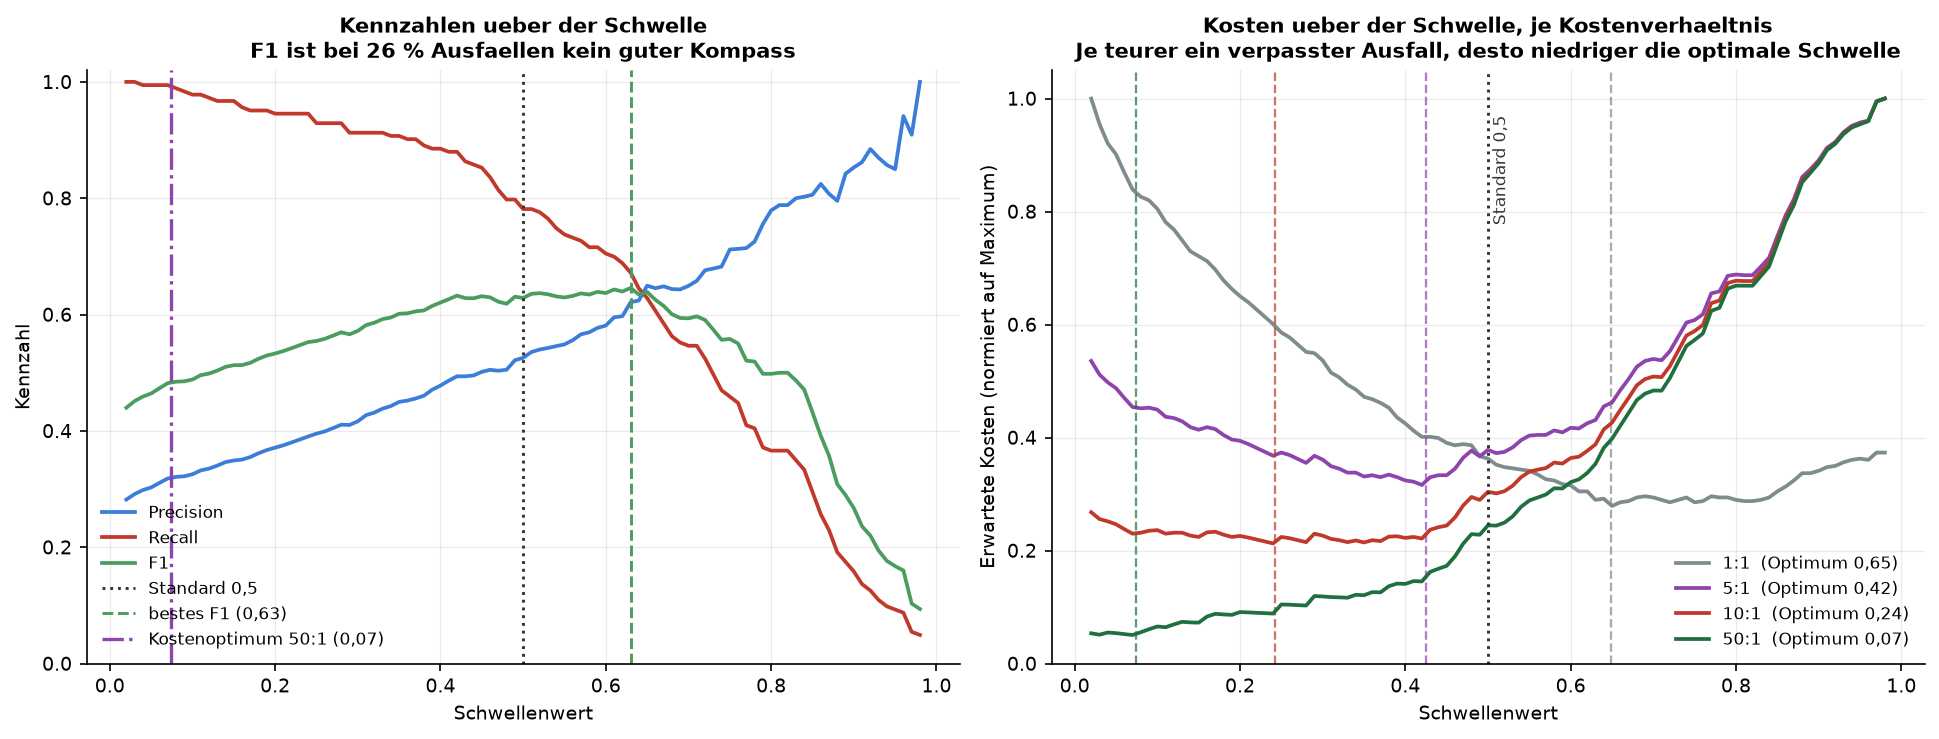
\includegraphics[width=0.90\linewidth]{07_schwellenwerte.png}
  \caption{Links: Precision, Recall und F1 ueber der Schwelle. Rechts: erwartete Kosten je Kostenverhaeltnis -- je teurer ein verpasster Ausfall, desto weiter wandert das Optimum nach links.}
\end{figure}


\begin{figure}[H]
  \centering
  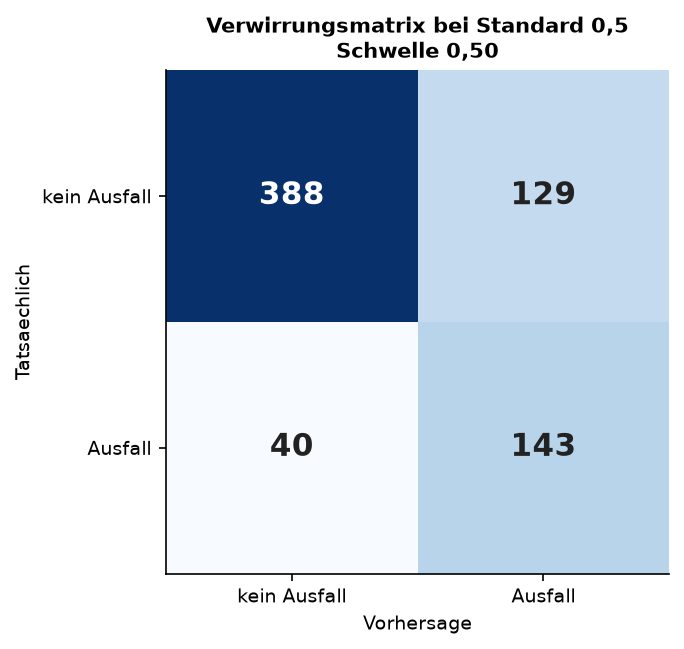
\includegraphics[width=0.55\linewidth]{08_konfusion_050.png}
  \caption{Verwirrungsmatrix bei der Standardschwelle 0,5.}
\end{figure}


\begin{figure}[H]
  \centering
  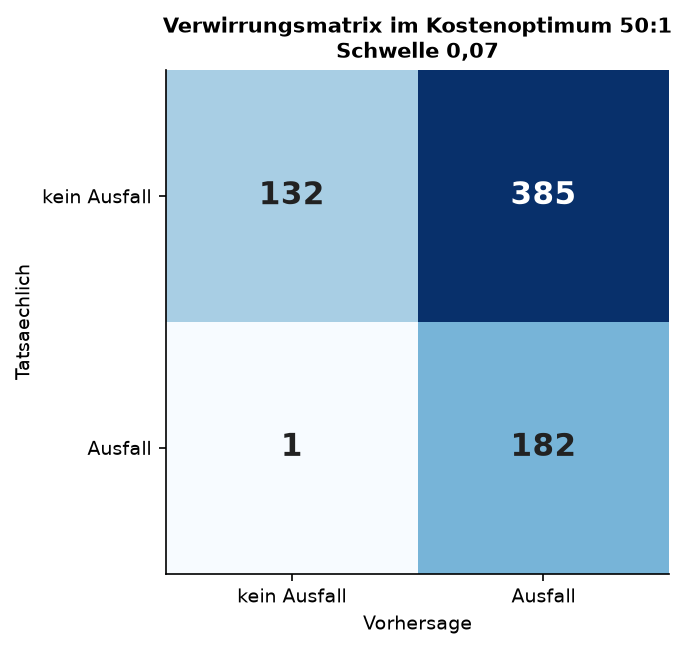
\includegraphics[width=0.55\linewidth]{09_konfusion_kosten.png}
  \caption{Verwirrungsmatrix im Kostenoptimum 50:1. Fast kein Ausfall wird mehr verpasst -- dafuer steigen die Fehlalarme.}
\end{figure}

